%! Author = charon
%! Date = 2/8/24

\subsection{Testen der Netzwerkschnittstelle über die Hardware}\label{subsec: hardware}
Um möglichst einfache Fehler bei der Emulation der Umgebung zu vermeiden, wurde die Hardware verwendet.
Das \gls{iot}-Gerät verfügt über einen Ethernet-Anschluss, über den eine direkte Verbindung zur Datenübertragung
hergestellt werden kann.\\
Um möglichst genaues Feedback über das Verhalten des Binarys zu erhalten, wurde sich über \gls{ssh} mit dem Gerät verbunden.
Danach wurde das Binary, welches für das Netzwerkprotokoll verantwortlich ist, beendet und in der Aktuellen \gls{ssh}-Session neu gestartet.
Beginnt man Daten an den Port 7142 zu senden, so erhält man auf der Konsole des \gls{iot}-Geräts folgende Ausgabe.
\begin{figure}[h]
    \frame{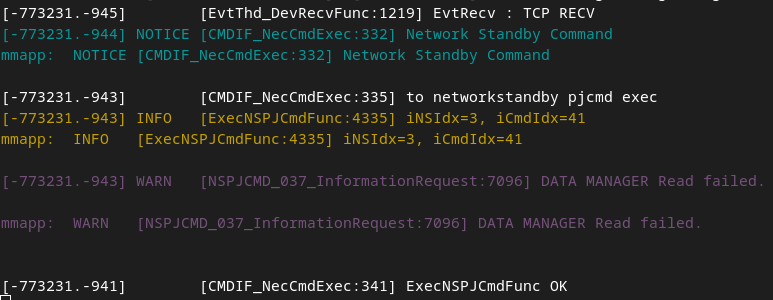
\includegraphics[width=\linewidth]{img/handler-cmd}}
    \caption{Beinhaltet die Ausgabe der Konsole nach händischem Starten des Binarys und Schicken eines Befehls an das Netzwerkprotokoll.}\label{fig:cmd-debug-info}
\end{figure}\\
Die Ausführung der Anfrage erfolgt über das Testskript \textit{binaryProt.py}~\cite{binaryProt-py}.
Das Testskript führt eine in der \texttt{main()} Funktion übergebene Funktion aus.
Es ist vorgesehen, dass alle Funktionen mit dem prefix \textit{exec} ausgeführt werden können.
Soll nur ein Befehl auf einem Gerät ausgeführt werden, so kann man die \gls{ip}-Adresse über die Konstruktoren mitgeben.
Die dokumentierten Funktionen sind bereits in menschenlesbarer Form in der Klasse \textit{Documented} enthalten.
Die Kommunikation über die Netzwerkschnittstelle erfolgt über einen Socket.
Hierzu wurde eine von Python bereitgestellte Bibliothek \textit{socket} verwendet.
Sie ermöglicht es dem Programmierer, unter Angabe einer \gls{ip}-Adresse und eines Ports, eine \gls{tcp}-Verbindung zu
einem Gerät aufzubauen.
Zur besseren Lesbarkeit wurde eine Hilfsfunktion geschrieben, welche den gesendeten Befehl in hexadezimaler Darstellung mit
einer kurzen Beschreibung der Funktionalität des Befehls in der Konsole ausgibt.
Zudem gibt das Programm die erhaltene Antwort des Befehls aus, die angibt, ob der gesendete Befehl erfolgreich auf dem
Gerät ausgeführt wurde.
Erkennbar ist die erfolgreiche Ausführung des Befehls, wenn das erste Byte der Antwort \textit{0x20}, \textit{0x21}, \textit{0x22}
oder \textit{0x23} entspricht.
Die Antworten sind ebenfalls zum Abgleich mit der Dokumentation des Protokolls~\cite{binary-prot-doc} gegenzuprüfen.
%! Author = chaorn
%! Date = 10.03.24

\begin{lstlisting}[caption={Ausgabe des implementierten Python-Skripts \textit{binaryProt.py}.
                            Es gibt den gesendeten Befehl in hexadezimaler Schreibweise,
                            sowie die \gls{ip}-Adresse des Geräts und die vom
                            Gerät gesendete Antwort aus.},label={lst:binary-prot-py-ausgabe}]
COMMAND DOCUMENTED: [base model type request] with bytes: 00 BF 00 00 01 00 C0
CHECKING IP-ADDRESS: 127.0.0.1
Sending 00 BF 00 00 01 00 C0
COMMAND SUCCESSFUL: 20 BF 01 40 10 00 FF 22 50 35 30 32 48 4C 00 00 00 00 13 FF 00 DE with checksum DE
\end{lstlisting}
Die Antworten der Befehle geben einen Hinweis darauf, dass es verschiedene Handler gibt, welche die Anfragen auf diesem Protokoll
bearbeiten.
Pahl dokumentierte die jeweiligen Handler, welche die Befehle auf dem Gerät bearbeiten, und ihre dazugehörigen Befehle
in einer Tabelle mittels des Python-Skripts~\cite{handler-table}.
Der Tabelle ist zu entnehmen, dass beim Untersuchen der Funktionen und ihrer Handler 53 dokumentierte Funktionen
vorliegen, wovon nur 26 eine valide Form besitzen.
Von diesen 26 Funktionen besitzen wiederum nur 15 einen Handler.
